\section{Analyse des besoins}

\subsection{Besoins fonctionnels}

Les besoins fonctionnels de la version Alpha sont regroupés dans le tableau~\ref{tab:besoins}.

\begin{table}[H]
\centering
\caption{Besoins fonctionnels de la version Alpha}
\label{tab:besoins}
\small
\begin{tabular}{p{0.07\textwidth}p{0.30\textwidth}p{0.53\textwidth}}
\toprule
\textbf{ID} & \textbf{Besoin} & \textbf{Description} \\
\midrule
BF1 & Authentification & Connexion du client et du fournisseur avec gestion de session et de rôle. \\
BF2 & Gestion des clients & Ajouter, modifier, rechercher et consulter les clients. \\
BF3 & Saisie des consommations & Saisir les index d'eau et d'électricité pour la période courante. \\
BF4 & Photos des compteurs & Téléverser une photo pour chaque compteur. \\
BF5 & Affichage du mois précédent & Afficher les index et les photos du relevé précédent. \\
BF6 & Détection des anomalies & Détecter un index inférieur ou un dépassement du seuil fournisseur. \\
BF7 & Confirmation ou correction & Permettre au client de confirmer une anomalie de seuil ou de corriger un index inférieur. \\
BF8 & Génération des factures & Calculer les montants et enregistrer la facture après validation. \\
BF9 & Consultation des factures & Afficher la liste et le détail des factures selon le rôle. \\
BF10 & Contrôle d'accès & Limiter chaque utilisateur à ses propres données ou à celles de ses clients. \\
\bottomrule
\end{tabular}
\end{table}

\subsection{Besoins non fonctionnels}

\begin{itemize}[leftmargin=*]
  \item \textbf{Sécurité} : requêtes préparées, protection CSRF, échappement HTML, contrôle des rôles et des uploads.
  \item \textbf{Fiabilité} : validation serveur des données et transactions pour les opérations multiples.
  \item \textbf{Maintenabilité} : séparation MVC, conventions de nommage et code organisé par module.
  \item \textbf{Utilisabilité} : interface claire, messages d'erreur explicites et navigation adaptée au rôle.
  \item \textbf{Responsive} : utilisation sur desktop, tablette et mobile.
  \item \textbf{Traçabilité} : conservation des consommations, photos, anomalies et factures.
\end{itemize}

\subsection{Règles métier}

\begin{itemize}[leftmargin=*]
  \item la saisie est ouverte du 18 du mois jusqu'au dernier jour du mois ;
  \item les index doivent être numériques et positifs ou nuls ;
  \item l'index courant doit être supérieur ou égal à l'index précédent ;
  \item un index supérieur au seuil du fournisseur déclenche une anomalie de seuil ;
  \item un index inférieur au relevé précédent impose une correction ;
  \item une anomalie de seuil peut être confirmée ou corrigée par le client ;
  \item une consommation validée ou une anomalie confirmée génère automatiquement une facture ;
  \item la TVA est fixée à 18 \% ;
  \item les tarifs sont appliqués par tranches progressives ;
  \item une consommation ne peut produire qu'une seule facture.
\end{itemize}

\subsection{Cas d'utilisation}

La figure~\ref{fig:usecase} présente le diagramme de cas d'utilisation du projet. La version Alpha couvre principalement l'authentification, la saisie des consommations, le traitement des anomalies et la gestion des clients. Les cas d'utilisation liés aux réclamations, à l'import annuel et aux paiements sont conservés dans la conception mais ne sont pas implémentés dans cette version.

\begin{figure}[htbp]
  \centering
  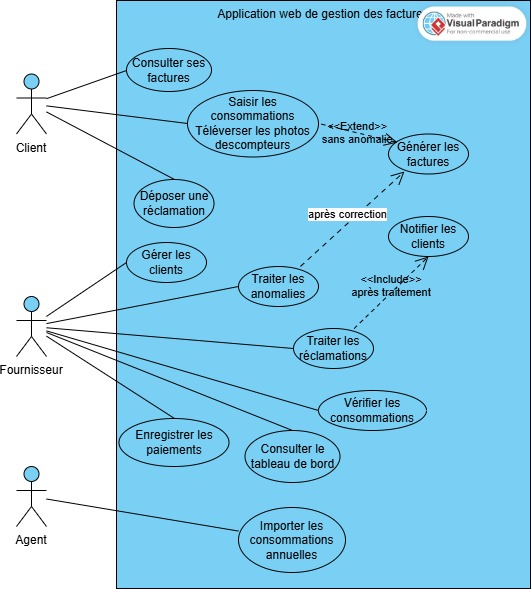
\includegraphics[width=0.60\textwidth]{../pdf/use_case_diagram.jpeg}
  \caption{Diagramme de cas d'utilisation du projet}
  \label{fig:usecase}
\end{figure}

\begin{table}[H]
\centering
\caption{Cas d'utilisation couverts par l'Alpha}
\label{tab:uc}
\small
\begin{tabular}{p{0.12\textwidth}p{0.36\textwidth}p{0.42\textwidth}}
\toprule
\textbf{Réf.} & \textbf{Cas d'utilisation} & \textbf{Acteur principal} \\
\midrule
UC01 & Saisir les consommations, téléverser les photos et générer la facture & Client \\
UC02 & Confirmer ou corriger une anomalie de saisie & Client / Fournisseur \\
UC04 & Gérer les clients (ajouter, modifier, rechercher) & Fournisseur \\
--- & Consulter les factures et leur détail & Client / Fournisseur \\
\bottomrule
\end{tabular}
\end{table}
